\subsection{Range Check}

In order to implement Range Check we are utilizing Lookup Argument technology. Please refer to Section \ref{sec:key-technologies} for detailed design. The basic fixed table is an 8-bit lookup table, i.e.\ 0-255. For 8-bit numbers, the validity is checked using Plookup. The utilization of Plookup check is shown in Figure \ref{fig:rangecheck-lookup}.
\begin{figure}[!ht]
    \centering
    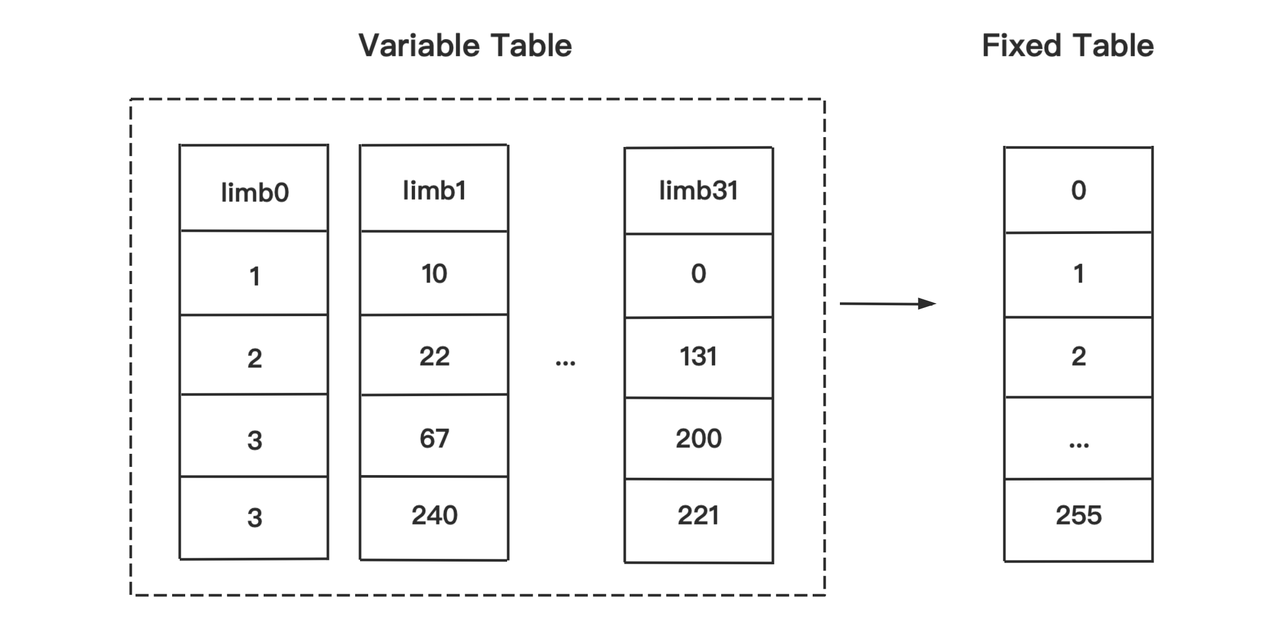
\includegraphics[width=0.8\textwidth]{rangecheck-lookup.png}
    \caption{Fixed/Variable lookup table}
    \label{fig:rangecheck-lookup}
\end{figure}

For numbers greater than 8 bits, break them down to multiple 8-bit limbs and perform Plookup respectively, and then check the constraints of sum and limbs. Take 256-bit as an example,
$\text{integer256} = \text{limb}_0 + \text{limb}_1 \cdot 2^8 + \text{limb}_2 \cdot (2^8)^2 + \text{limb}_3 \cdot (2^8)^3 + \cdots + \text{limb}_{31} \cdot (2^8)^{31}$.
